\subsection{EMCal trigger rejection factor}
The electron yield obtained using the EMCal triggered
data sample is enhanced at high $p_{\rm T}$, and is corrected by the trigger rejection factor (RF). The RF quantifies the fraction of MB interaction triggers which are rejected by the  EMCal trigger condition. It was
obtained via a data-driven method using the ratio of the cluster energy distribution in triggered-data to the one in minimum-bias triggered data, which gives the turn-on curve. The turn-on curve is determined in multiplicity integrated and in different multiplicity intervals in pp and \pPb collisions. Figure~\ref{fig:RF} shows an example of the turn-on curve for multiplicity integrated pp and \pPb collisions for both trigger energy thresholds (EG1 and EG2).

\begin{figure}[h!]
    \centering
    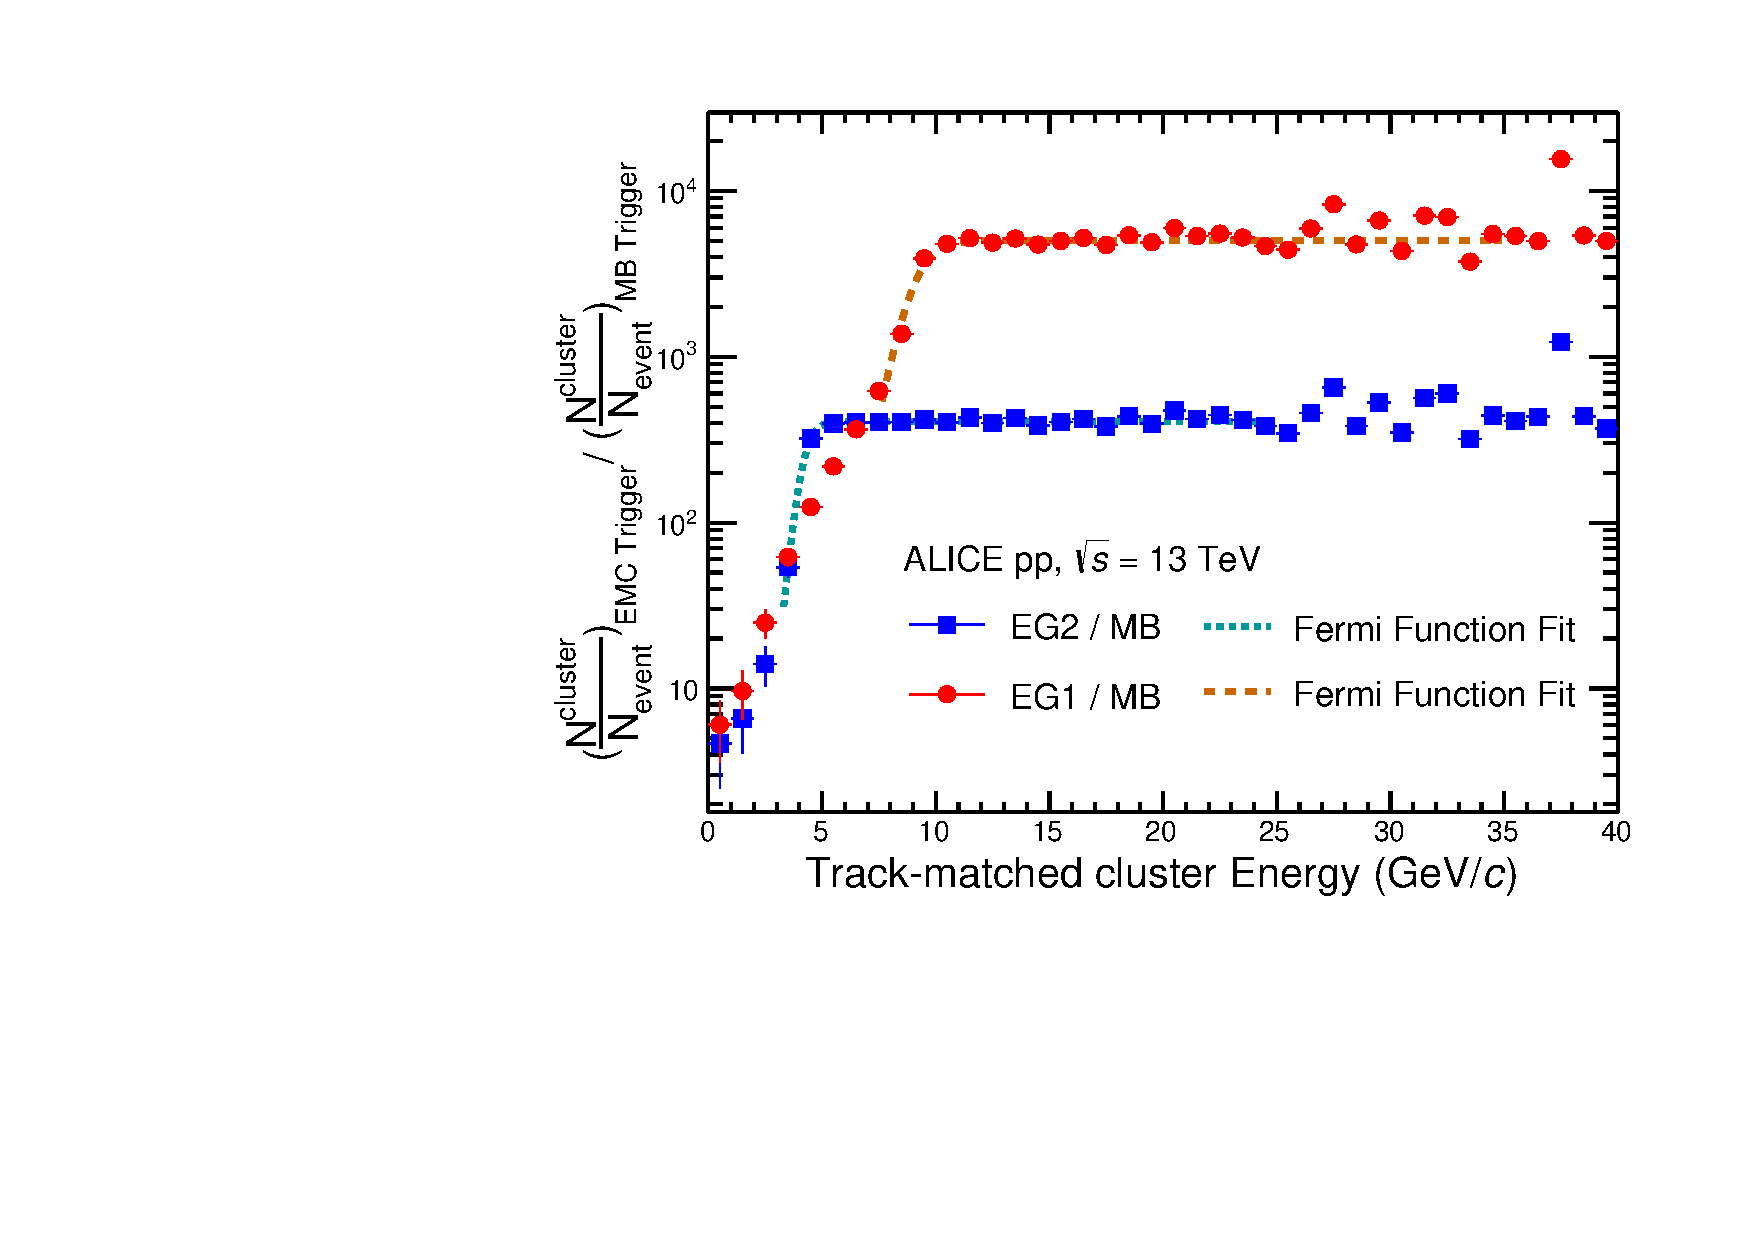
\includegraphics[width=0.48\linewidth]{{figures/Results/HFE_ppNormalB/RF_trackmatchCluster}.pdf}
    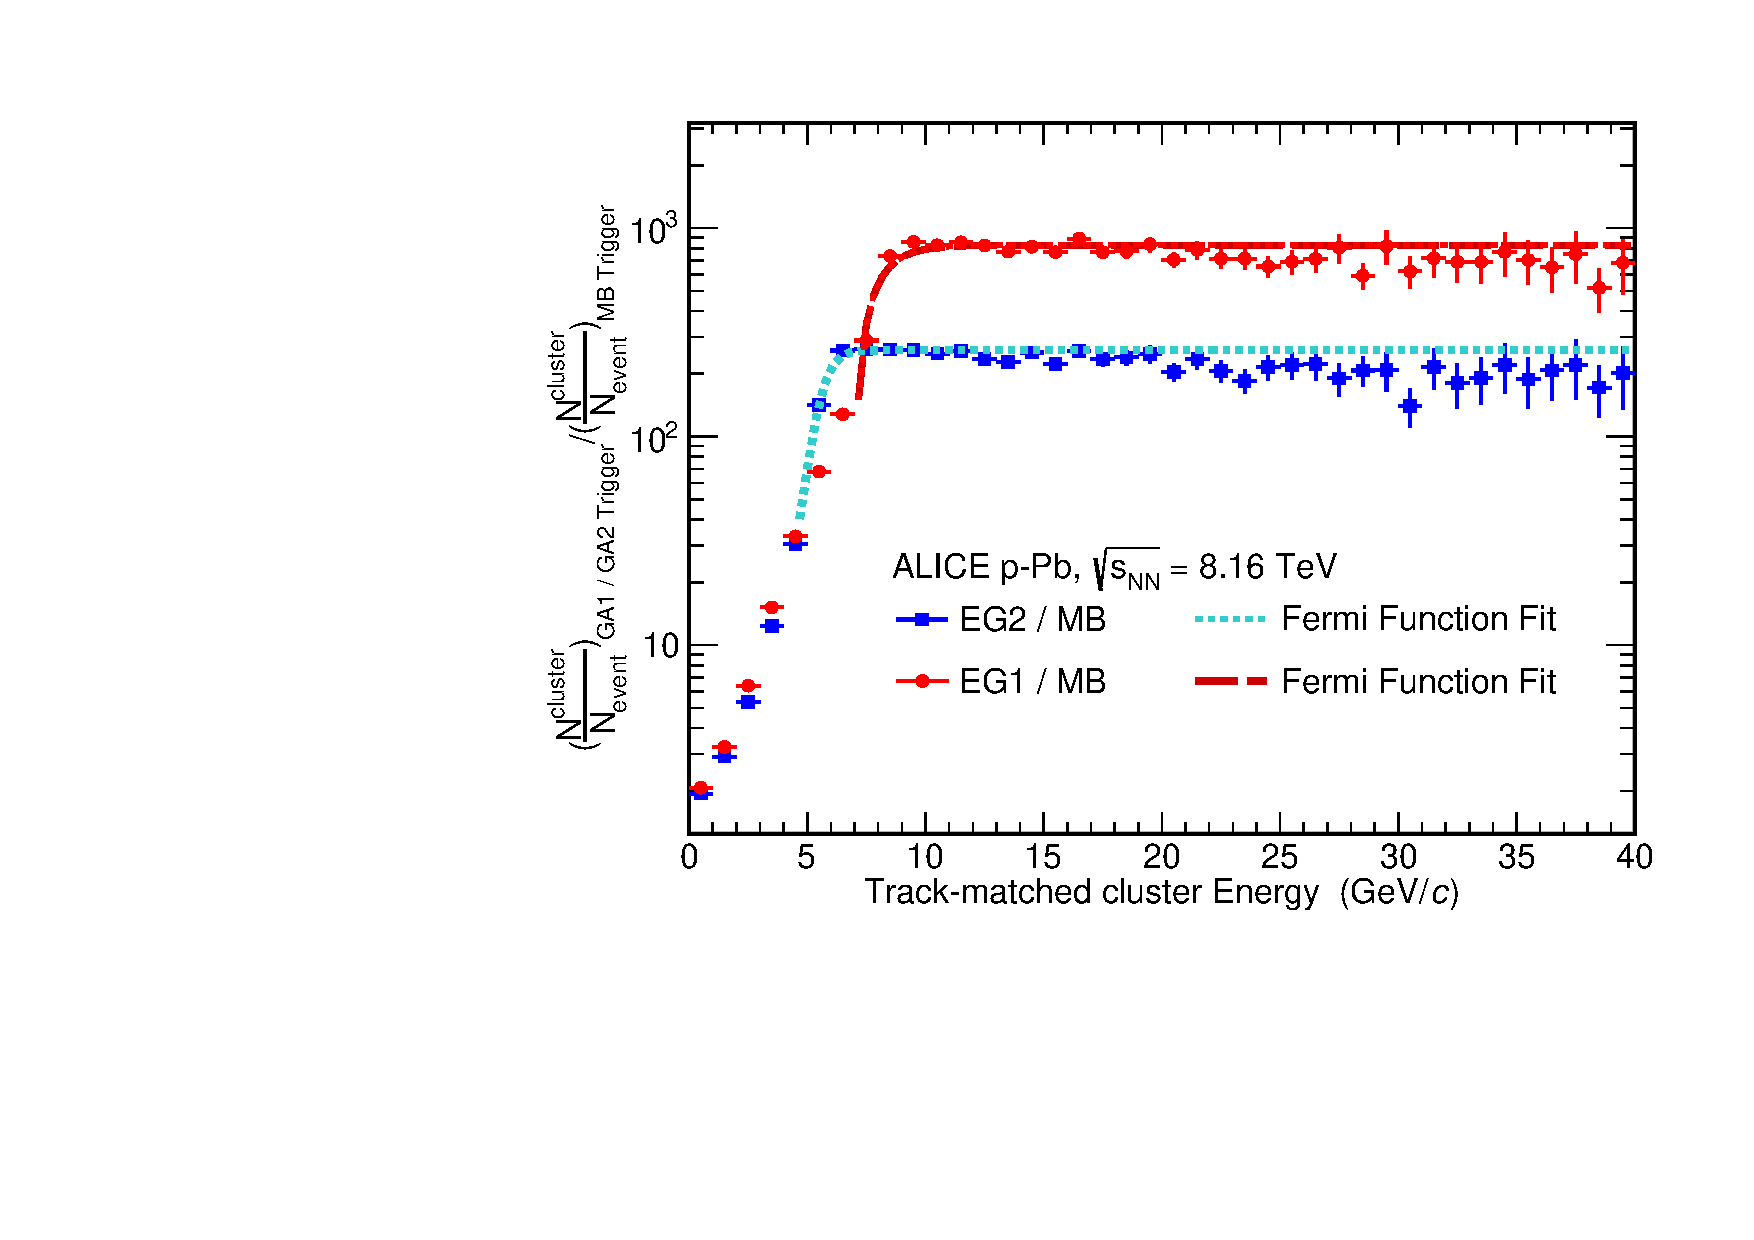
\includegraphics[width=0.48\linewidth]{figures/Results/HFE_pPb/RF_extendedpT_extendedFit.pdf}
    
    \caption{Trigger Rejection Factor for EG2 and EG1 triggers in pp collisions at $\sqrt{s}=13$ TeV (left) and in \pPb collisions at $\sqrtsNN = 8.16$ TeV (right).}
   \label{fig:RF}
\end{figure}


The rejection factor was obtained by fitting a Fermi function~\cite{Fermi:1934hr, Wilson:1968pwx} to the turn-on curve from around the trigger threshold up to higher $p_{\rm T}$ where the distribution flattens. The values obtained for the rejection factor are summarised in Table~\ref{table:RF}. The uncertainties on the values of the rejection factor were obtained using different fit ranges on the plateau.

\begin{table}[h!]
\caption{Multiplicity integrated values of the EMCal trigger rejection factor with their uncertainties for the EG2 and EG1 triggered datasets in pp and \pPb collisions.}
    \centering
    \begin{tabular}{c| c c | c c}
    \toprule
    \multicolumn{1}{c|}{}&
    \multicolumn{2}{c|}{pp $\sqrt{s} = 13 \TeV$}& \multicolumn{2}{c}{\pPb $\sqrt{s_{\rm NN}} = 8.16 \TeV$}\\
%   \midrule
   %    &  &  pp &  & p--Pb\\
                Trigger   & EG2 & EG1 & EG2 & EG1 \\
                \midrule
     RF value & { 406 $\pm$ 12 } & { 5040 $\pm$ 202 } &  255.65 $\pm$ 1.50 & 815.76 $\pm$ 8.43 \\
     \bottomrule
    \end{tabular}
    \label{table:RF}
\end{table}


\subsection{Efficiency correction and normalization}\label{section:corrections}
The raw number of electrons from heavy-flavour hadron decays obtained after the subtraction of hadron contamination, photonic and other background contribution, is divided by the number of events analysed (${N_{\rm events}}$), 
%by the value of $p_{\rm T}$ at the centre of each bin and 
 width of the $\pt$ range ($\Delta p_{\rm T}$), by the width $\Delta y$ of the covered rapidity interval, by the geometrical acceptance ($\epsilon^{\rm geo}$) times the track reconstruction ($\epsilon^{\rm reco}$) and electron identification efficiencies ($\epsilon^{\rm eID}$) and a factor of two to obtain the charge averaged invariant differential yield which is further multiplied by minimum bias trigger cross section to get the $p_{\rm T}$-differential production cross section of electrons. The MB trigger cross section for pp collisions at $\sqrt{s}$ $= 13$ TeV and for \pPb collisions at $\sqrt{s_{\rm{NN}}}$ $=8.16$ TeV was $\sigma_{\rm MB}$ $=$ 57.8 $\pm$ 2.9 mb and 2100 $\pm$ 60 mb respectively.  
 %{\color{blue} (is this value same for both lowB and normal B?) {(\color{cyan} Yes, at the moment it is taken to be same)} and {\color{teal} 2100 $\pm$ 60 mb}} respectively.  

\begin{equation}
 \frac{d^2\sigma}{dp_{\rm T}dy} = \frac{1}{2}  \frac{1}{\Delta y \Delta p_{\rm T}} \frac{{N_{\rm{raw}}}} {\epsilon^{\rm{geo}} \times \epsilon^{\rm reco} \times  \epsilon^{\rm {eID}} } \frac{\sigma_{\rm{MB}}}{N_{\rm {events}}}
%\frac{1}{2 \pi p_{\rm{T}}} \frac{d\sigma}{dp_{\rm T}dy} = \frac{1}{2} \frac{1}{2 \pi {p_{\rm T}^{\rm centre}}}  \frac{1}{\Delta y \Delta p_{\rm T}} \frac{{N_{\rm{raw}}}} {\epsilon^{\rm{geo}} \times \epsilon^{\rm reco} \times  \epsilon^{\rm {eID}} } \frac{\sigma_{\rm{MB}}}{N_{\rm {events}}} 
\end{equation}

The above mentioned acceptance and track reconstruction efficiencies were computed using MC simulations. In pp and \pPb analyses, the MC sample was obtained using PYTHIA 6~\cite{Sjostrand:2006za} and HIJING~\cite{Wang:1991hta} event generators respectively, with the generated particles propagated through the ALICE apparatus using GEANT 3~\cite{Brun:1073159}.  To increase the sample of electrons from charm- and beauty-hadron decays, a sample of charm and beauty quarks generated with PYTHIA 6 is embedded into each MC event. The electron identification (eID) efficiency for TOF, TPC and the EMCal detectors were obtained separately, and then multiplied according to the detectors used in the analysis to compute the full eID efficiency $\epsilon^{\rm eID}$. The eID efficiency of TOF detector was obtained using the above mentioned MC sample and was found to be 60--70$\%$ (40--65$\%$) for  0.5 $<$ $p_{\rm T}$ $<$ 1.5 GeV/c increasing upto 75$\%$ (70$\%$) at 4 GeV/c in low (nominal) B analysis. The TPC eID efficiency was determined using a data-driven approach based on the $n^{\rm{TPC}}_{\sigma,\rm{e}}$ distribution~\cite{Abelev:2012xe}, and was found to be $\sim 88\%$ at $p_{\rm T}= 0.2$ GeV/$c$, increasing to $\sim 89\%$ at $p_{\rm T} > 0.5$ GeV/$c$ for $-1 < n^{\rm{TPC}}_{\sigma,\rm{e}}< 3$ range, for low B data sample. In nominal B dataset, it is found to be $\sim 86\%$ at $p_{\rm T}= 0.5$ GeV/$c$ and $\sim 88\%$ at $p_{\rm T} > 4$ GeV/$c$ for $-1 < n^{\rm{TPC}}_{\sigma,\rm{e}}< 3$ range. In \pPb dataset, similar TPC eID efficiency is observed. It is found to be be $\sim 86\%$ at $p_{\rm T}= 0.5$ GeV/$c$ and $\sim 89\%$ at $p_{\rm T} > 4$ GeV/$c$ for $-1 < n^{\rm{TPC}}_{\sigma,\rm{e}}< 3$ range.  The eID efficiency with EMCal, employing the $E/p$  and shower shape cut was estimated using Monte-Carlo simulations. It was found to be $\sim$ 60\% at 3 GeV/$c$ increasing upto $\sim$ 80 \% at 10 GeV/$c$ and at higher \pt for pp collisions. 
%The product of the overall acceptance and efficiency ($\epsilon^{\rm geo} \times \epsilon^{\rm reco} \times \epsilon^{\rm eID}$) as function of $p_{\rm{T}}$ for the TPC-TOF analysis and for the TPC-EMCal analysis are shown in Figure~\ref{Fig:TotEffi} for both pp and \pPb collisions.
The total reconstruction efficiency ($\epsilon^{\rm{geo}} \times \epsilon^{\rm reco} \times  \epsilon^{\rm {eID}}$) for different data sets and with different detectors are presented in Figure~\ref{Fig:ppHFEEff}. Due to better track matching between TPC and TOF detectors with low magnetic field, a higher reconstruction efficiency was observed in low B data sample compared to the nominal B field sample.

\begin{figure}[!ht]


 \begin{center}
      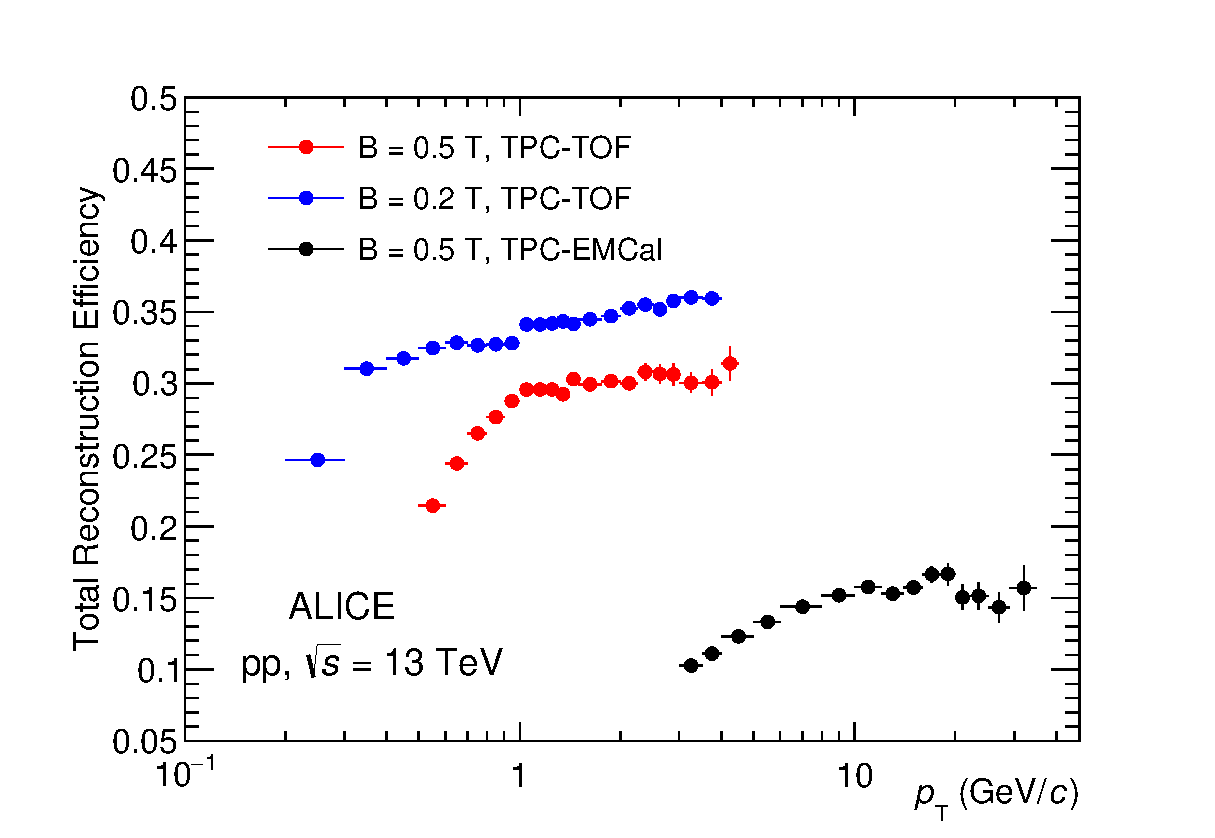
\includegraphics[width=0.48\linewidth]{figures/Results/HFE_pp_LowB/CompWithNormalB_LowB_logx.eps}
      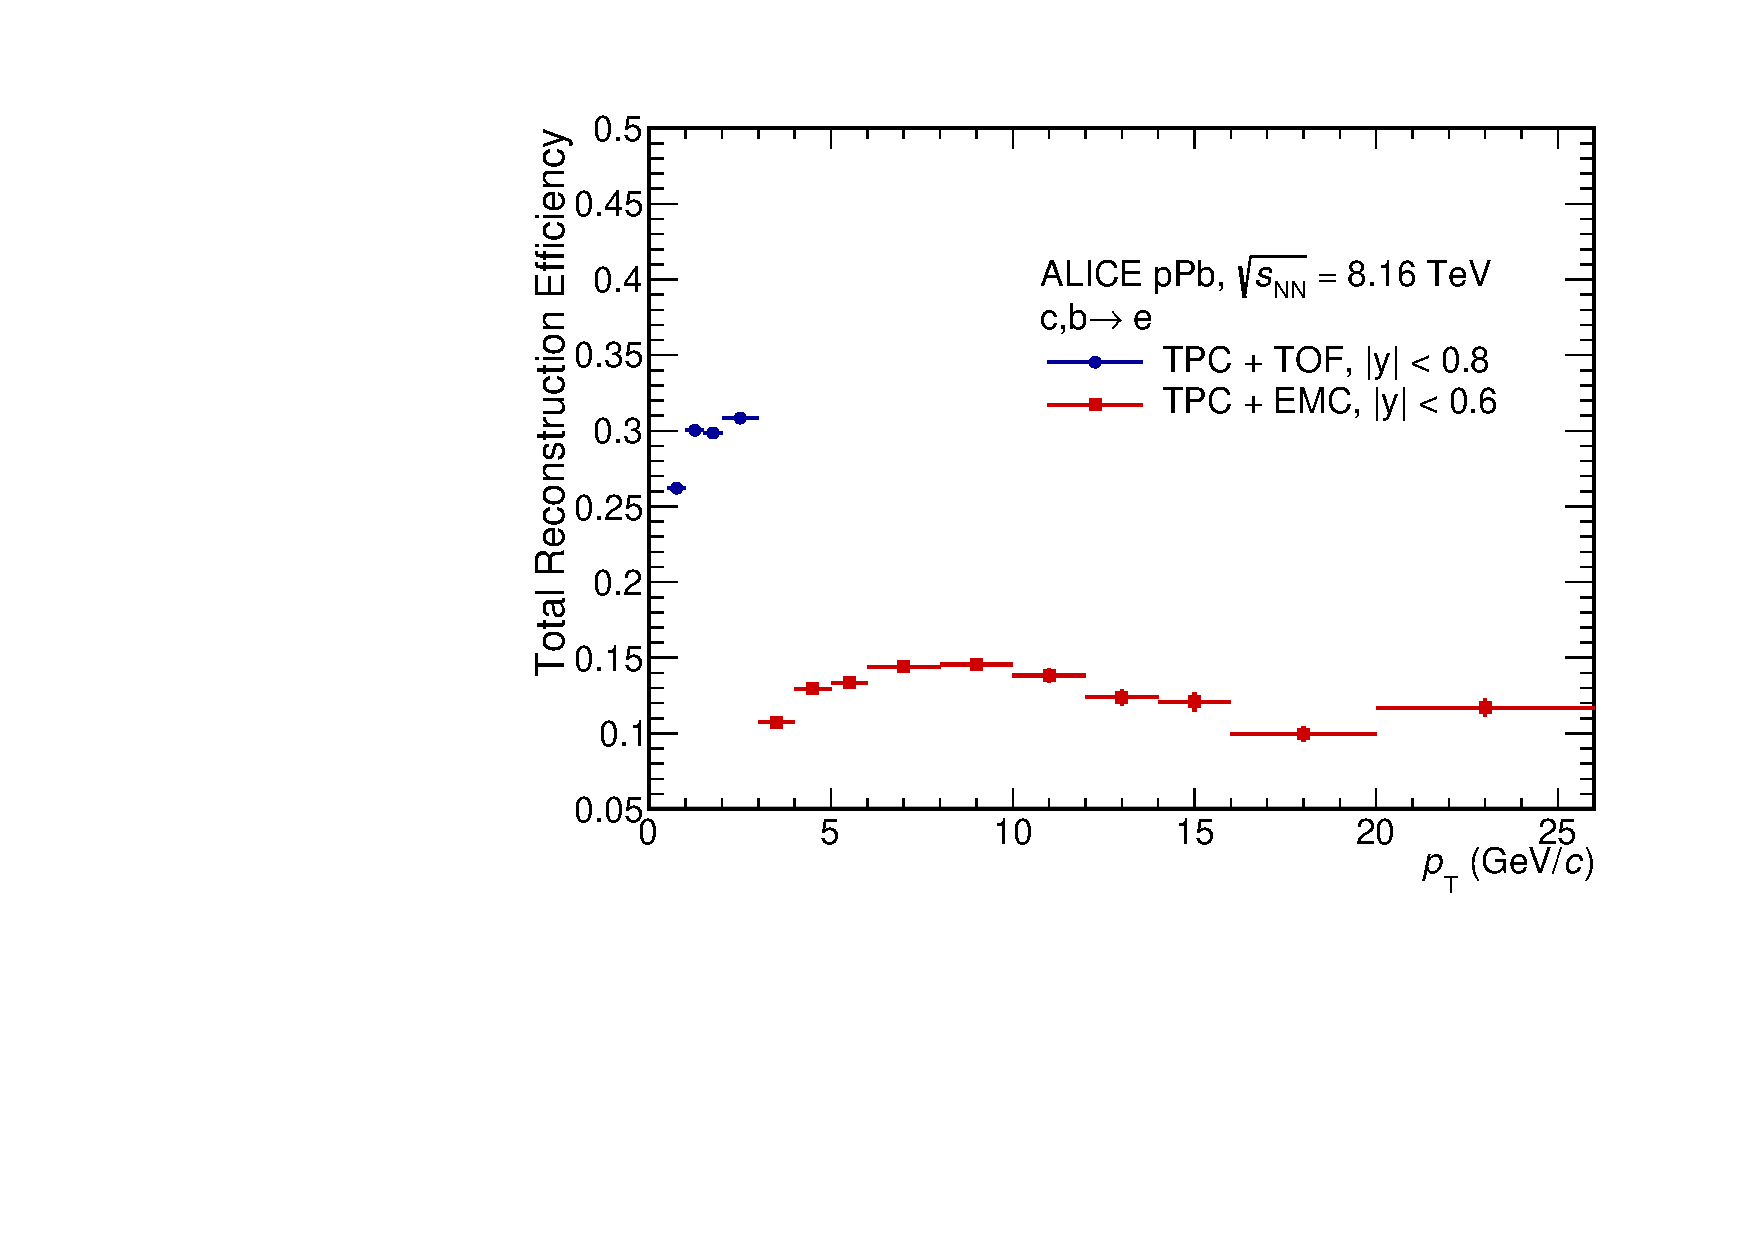
\includegraphics[width=0.46\linewidth]{figures/Results/HFE_pPb/TotalReconstructionEfficiency.pdf}
      \end{center}

\caption{Total reconstruction efficiency of electrons from heavy-flavour hadron decays in pp collisions at $\sqrt{s}$ $=$ 13 TeV with normal and low magnetic field using TPC-TOF and TPC-EMCal (left) and in \pPb collisions $\sqrtsNN=8.16$ TeV using TPC-TOF and TPC-EMCal (right).}        
\label{Fig:ppHFEEff}
\end{figure}


%Dedicated MC simulations are used to determine the efficiencies. For pp analysis, each event is embedded with one $c\bar{c}$ or $b\bar{b}$ pair decaying semileptonically in heavy-flavour enriched PYTHIA MC sample. HIJING event generator is used for p--Pb analysis in which heavy-flavour signal is added using PYTHIA.